% article example for classicthesis.sty
\documentclass[10pt,a4paper]{article} % KOMA-Script article scrartcl
\usepackage{lipsum}
\usepackage{url}
\usepackage[nochapters]{classicthesis} % nochapters
\usepackage{amsmath}
\usepackage{multirow}
\usepackage{graphicx}
\usepackage{dsfont}

% for algorithm description
\usepackage{alltt}
% for algorithm description in a box
\usepackage{boxedminipage}

\DeclareMathOperator*{\argmin}{argmin}

\begin{document}
	\pagestyle{plain}
	\title{\rmfamily\normalfont Thompson Sampling \\in Adversarial Environments}
	\author{Travis Dunlop }
	\date{July 3, 2018\\ $\,$ 
			 \\Advisors: Gergely Neu, Mihalis Markakis} 
	
	\maketitle
	
	\begin{abstract}
		Thompson Sampling is an increasingly popular family of algorithms for decision making in online optimization.  And, this is for good reason.  If the loss of each action is independent and identically distributed, the external regret is bounded by $\mathcal{O}(\ln T)$ (where $T$ is total time steps) \cite{agrawal}. This rivals the performance of state-of-the art algorithms.  However, what is not yet understood is it's performance if the losses are not iid.  In this thesis, we provide empirical evidence that Thompson Sampling performs as well as algorithms with tight regret bounds in adversarial environments.  This evidence comes from constant sum game play as well as evolutionary strategies.
	\end{abstract}
	
	\section{Introduction}
	
	In 1933, William R. Thompson came up with Thompson Sampling \cite{original_gangster} while researching the best way treat patitents with novel medicines.  Consider a scenerio where patients with the same ailment come to a doctor over time.  The doctor has a number of medicines she could prescribe.  She has prescribed some of them many times before and knows how well they work.  But she faces a dilema: should she try out a new medicine? It could work even better than the others, or perhaps even worse.  She needs to balance the need to \textit{explore} the possibilities with \textit{exploiting} the treatments she knows work well.  How should she prescribe medicine such that negative health outcomes are minimized?
	
	Thompson's answer to this question is a Bayesian approach.  For each of the medicines, the doctor has a prior belief on the effect.  This is expressed as a probability distribution over the health outcomes.  As she prescribes the medicines, her beliefs are updated.  To make a decision, she samples a value from each of the distributions and chooses the one with minimum sampled loss.  The probability distribution over the health outcomes captures her uncertainty about the true distribution as well as the inherent randomness of the problem.  Sampling from these distributions allows for each medicine to be chosen in proportion to her belief of it's quality.  Exploration is induced by chosing the appropriate prior for medicines whose effects have not yet been seen.
	
	Thompson Sampling is known to perform well in the case where a patient's reaction to the medicines are independent from each other and identically distributed.  Unfortunately, in many situations there is no guarantee that this assumption holds.  Perhaps the population grows resistent to a treatment, or environmental factors change it's efficacy.  Thus, we would like to know how robust is Thompson Sampling when the data is not iid.  What is common in literature, is to analyze the worst case scenerio - when the losses are not just non-iid, but they are set by an adversary who specifically tries induce poor performance.  If an algorithm works well not just in easy situations, but in these adversarial cases, then it is one worth investing in.
	
	Now we give an overview of the rest of the document.  We will first give a more explicit mathematical description of the problem at hand.  Then, we describe the particular flavor of Thompson Sampling we analyze.  Next, we discuss other algorithms which have been used to tackle this problem.  After, we recast this problem within game theory and leverage some theoretical results to estimate the regret of these algorithms.  Finally, we use an evolutionary strategy to maximize the regret on these algorithms and report the results.
	
	\section{Problem Setup}
	
	We consider a version of the 'prediction with expert advice' framework from the textbook \textit{Prediction, Learning, and Games} \cite{PLG}.  In this setup, there is a forecaster (analagous to the doctor) that plays a repeated game against their adversary - the environment.  
	
	First, the environment choses a loss for each action and time step $\ell_{i, t}$.  Where $i \in \{1, 2, ... N\}$ corresponds with the possible actions  of the forecaster and $t \in \{1, 2, ..., T\}$ is the timestep.  Then, the forecaster plays the game.  For each timestep $t$: the forecaster chooses an action $a_t \in \{1, ..., N\}$, and incurrs loss $\ell_{a_t, t}$.  The losses for all actions are then revealed to the forecaster. 
	
	The forecaster tries to learn from the losses it's seen to choose good actions and the environment tries to trick the forecaster into incurring high loss.  This setup can be thought of as a mulit-armed bandit problem with full information.
	
	Note, we are cheating here compared with the story of the doctor.  When the doctor chooses medicines, she only observes the effect of the medicine she chose.  By assuming we have full information, we assume we know what would have happened had the doctor chosen another medicine.  We do this for mathematical ease.  If we are able to prove a regret bound in this easier framework, it will be a much smaller step to prove it in the harder one.  \\
	
	\noindent \begin{minipage}{\textwidth}
	\centerline{\textbf{Problem Framework}} 
	\noindent\begin{boxedminipage}{\textwidth}
		\textbf{Parameters}: Number of actions: $N$, Number of timesteps: $T$ \\
		Environment chooses losses $\ell_{i, t} \in [0, 1]$ for $i \in \{1, 2, .., N\}$ \& $t \in \{1, 2, ..., T\} $ \\
		\textbf{For each timestep} $t = 1, 2, ..., T$
		\begin{enumerate}
			\item Forecaster chooses action $a_{t} \in \{1, 2, ..., N\}$
			\item Environment reveals losses for each action $\ell_{i, t}$ for $i \in \{1, 2, ..., N\}$
			\item Forecaster suffers loss of chosen action $\ell_{a_t, t}$
		\end{enumerate}
	\end{boxedminipage}
\end{minipage}
	\\ $\,$ \\
	Now, we need some way of scoring the game between the forecaster and environment.  At first glance, a natural choice is the cummulative loss of the forecaster: $\widehat{L} = \sum_{t = 1}^{T} \ell_{a_t, t}$.  However, this gives too much power to the environment.  They could simply maximize loss by choosing $\ell_{i, t} = 1$ for all actions and time steps.
	
	A better choice of metric is regret. We compare what the forecaster did with what would have been a good action in hindsight.  While there are several forms of regret, here we consider \textit{external} regret - the difference between the forecasters loss and that of the best fixed action:
	$$R_T = \widehat{L}_T - L^*_T$$
	Where $L^* = \min_j \sum_{t = 1}^{T} \ell_{j, t}$ is the loss of the best fixed action.  
	
	The ultimate goal of this work is to find a tight upper bound on the expected regret, maximized with respect to the losses the adversary could choose:
	
	$$ \max_\ell E [R_T] $$
	
	\section{Thompson Sampling}
	
	Since we are considering a framework where the losses are bounded between 0 and 1, we choose to analyze the popular Beta-Bernoulli variant of Thompson Sampling.  In this case we assume that the losses, $\ell_{i, t}$, are Bernoulli distributed with probibility they are equal to one is $\theta_{i, t}$.
	
	$$\overset{posterior}{\underset{beta}{P(\theta_{i, t} | \ell_{i, t})}} = 
		\overset{liklihood}{\underset{bernoulli}{P(\ell_{i, t} | \theta_{i, t})}} \, 
		\overset{prior}{\underset{beta}{P(\theta_{i, t})}}$$
	
	Recall that for a random variable $\theta \sim \text{Beta}(\alpha, \beta)$, the density is $P(\theta = x) \propto x^\alpha (1 - x)^{\beta-1} $.  Here, $\alpha$ and $\beta$ are shape parameters.  The higher the value of $\alpha$ the more the density is shifted towards one, the higher $\beta$ the more of a shift towards 0.  Thus, this leads to a straightforward update rule.  If we observe $\ell_{i, t} = 1$, we add one to our current estimate of $\alpha_i$, if we observe $\ell_{i, t} = 0$ we add one to $\beta_i$.  Of course, by default this just supports $\ell_{i, t} \in \{0, 1\}$ and not $\ell_{i, t} \in \left[ 0, 1 \right]$.  In order for the algorithm to support values between 0 and 1, we introduce a secondary loss $\widetilde{\ell}_{i, t}$ which is Bernoulli distributed according to the primary loss.  Thus, the probability of updating the parameter is in proportion to the level of the observed loss.  This rule is shown in item three of the boxed explanation below.
		
	\centerline{\textbf{Thompson Sampling: Beta-Bernoulli}} 
	\noindent\begin{boxedminipage}{\textwidth}
		Set parameters $\alpha_i = 1$ and $\beta_i = 1$ for all $i \in \{1, ..., N\}$\\
		\textbf{For each timestep} $t = 1, 2, ..., T$
		\begin{enumerate}
			\item Sample $\theta_{i, t} \sim \text{Beta}(\alpha_i, \beta_i)$ and choose action $a_t = \argmin_i \theta_{i, t}$
			\item Observe losses $\ell_{i, t}$ for $i \in \{1, 2, ..., N\}$
			\item Perform Bernoulli trial for each action: $\widetilde{\ell}_{i, t} \sim \text{Bernoulli}(\ell_{i, t})$
			\item $
			\begin{aligned}			
			\text{Update parameters: } \alpha_i &= \alpha_i + \widetilde{\ell}_{i, t} \\
			\beta_i &= \beta_i + 1 - \widetilde{\ell}_{i, t}
			\end{aligned}
			$
		\end{enumerate}
	\end{boxedminipage}

	For a more thorough treatment of Beta-Bernoulli Thompson Sampling, please refer to \cite{agrawal}
	
	
	\section{Other Algorithms}
	
	Of course, Thompson Sampling is not the only algorithm that could be used in this 'prediction with expert advice' framework.  In this section we discuss two of the more popular strategies.  Both of them have provable bounds on adversarial regret.
	
	\subsection{Follow the Perturbed Leader}
	
	The first of these algorithms is based of the idea of 'following the leader'.  That is, choose the action which has the lowest cummulative loss so far.  However, it is well known result that in this most naive implementation, one can construct losses such that the regret grows linearly with time.
	
	To see this imagine two actions with losses (1, 0, 1/2, 0, 1/2, 0, ) (1, 1/2, 0, 1/2, 0, 1/2...).
	
	These adversarial cases inspired the creation of, follow the \textit{perturbed} leader (FPL).  That is to choose the action with the lowest cummulative so far, but perturbed by some random noise.
	
	$$a_t = \argmin_i L_{i, t-1} + Z_{i, t}$$
	
	There are many choices one could make for the distribution of this perturbation and thus many variants of the algorithm.  For example, it could be uniformly or exponentially distributed, or perhaps follow a random walk, or even follow a dropout pattern.  The citations and regret bounds for these variants are in the table below.
	
	\subsection{Exponential Weighted Averaging}
	
	Another popular algorithm for this problem is the exponential weighted averaging (EWA).  In this scheme, the probability of choosing an action is in proportion to the exponential of the cummulative loss thus far. 
	
	$$P(a_t = i) = \frac{e^{-\eta_t L_{i, t - 1}}}{\sum_{j = 1}^N  e^{-\eta_t L_{j, t - 1}}}$$
	
	Where $\eta_t$ is a learning rate parameter.  The main ways of varying this algorithm is by choosing different values for this parameter.  Some of these rely on having more information about the system.  For example the fixed learning rate $\eta = \sqrt{8 (\ln{N})/T}$ relies on knowing the time horizon $T$ a priori.  Ideally we want an algorithm that both has a tight regret bound with as little extra information needed as possible.
	
	\subsection{Comparison of Algorithms}
	
	\begin{table}[h!]
		\centering
			\makebox[\textwidth]{\begin{tabular}{cccc}
				Algorithm & Type & Adversarial Regret Bound & Citation\\
				\hline
				\multirow{4}{*}{Exponential Weighted Average}
				&$\eta_t = \sqrt{8 (\ln{N})/t}$&$\mathcal{O}(\sqrt{T \, \log{N}} + \log{N})$ & Section 2.3 \cite{PLG}\\
				&$\eta = \sqrt{8 (\ln{N})/T}$&$\mathcal{O}(\sqrt{T \, \log{N}})$ & Section 2.2 \cite{PLG}\\
				&$\eta_t = \min \{ 1, C \sqrt{(\ln{N}) / \text{Var}(\widehat{L}_t)} \}$ &$\mathcal{O}(\sqrt{\text{Var}(\widehat{L}_T) \, \log{N}} + \log{N})$ & Equation 13 \cite{eq13}\\
				&AdaHedge&$\mathcal{O}(\sqrt{L^* \, \log{N}} + \log{N})$ & \cite{adahedge}\\
				\hline
				\multirow{4}{*}{Follow the Perturbed Leader}

				&Uniform&$\mathcal{O}(\sqrt{TN})$ & Corollary 4.4 \cite{PLG}\\
				&Random Walk&$\mathcal{O}(\sqrt{T \, \log{N}} + \log{T})$ &\cite{random_walk}\\
				&Exponential&$\mathcal{O}(\sqrt{L^* \, \log{N}} + \log{N})$ & Corollary 4.5 \cite{PLG}\\
				&Dropout&$\mathcal{O}(\sqrt{L^* \, \log{N}} + \log{N})$ &\cite{dropout}\\
				\hline
			\end{tabular}}

		\label{tab:multicol}
	\end{table}



	\section{Constant Sum Games}
	
	In order to come up with ways to generate adversarial data, we now turn to game theory - specificially, constant sum games.  In this setup, there are two players: the row player and the column player.  Here we are talking about the rows and columns of a payoff matrix $P \in \mathds{R}^{N \times N}$.  At each round the row player chooses a row $i \in \{1, ..., N\}$ and the column player chooses a column $j \in \{1, ..., N\}$.  The row player incurrs a loss $P_{i, j}$ while the column player loses $c - P_{i, j}$.  Since we want to keep losses for both players bounded on the range $\left[ 0, 1 \right] $ we will say $P \in \left[ 0, 1 \right] ^{N \times N}$ and $c = 1$.
		
	In the figure on the next page we visualize the outcomes of many repeated trials.  Each column of the plots show a different value of $N$.  The rows are payoff matrices.  We consider three types: 
	\begin{itemize}
		\item identity - in this setup, the row player wants to choose the same action as the column player.  The column player wants the opposite.  Here is an example matrix:
		$$
		\begin{bmatrix}
			1  &  0 & 0     \\
			0  &  1 & 0     \\
			0  &  0 & 1     \\
		\end{bmatrix}
		$$
		\item rock paper scissors - In the three by three case this is exactly the game of rock paper scissors.  Each row or column refers one of the three actions.  Paper beats rock, rock beats scissors, scissors beats paper.  Note here the losses are rescaled to be between zero and one.
		$$
		\begin{bmatrix}
			0.5  &  0 & 1     \\
			1  &  0.5 & 0     \\
			0  &  1  & 0.5    \\
		\end{bmatrix}
		$$
		\item uniform - In this setup, each entry of the payoff matrix is generated uniformly at random.
	\end{itemize}
	We compare three algorithms: 
	\begin{itemize}
		\item Beta-Bernoulli Thompson Sampling
		\item Exponential weighted averaging (EWA) - with learning rate $\eta_t = \sqrt{8 (\ln{N})/t}$
		\item Follow the perturbed leader (FPL) with dropout perturbations -  we say $\widetilde{\ell}_{i, t} = 1$ with probability $(1 - \alpha) \ell_{i, t}$ where $\alpha \in (0, 1)$.  Decisions are made by choosing the lowest cummulative loss of $\widetilde{\ell}_{i, t}$
	\end{itemize}

	For each combination of $N, T$, payoff matrix and algorithm we play 100 rounds of the game.  The point plotted is the maximum regret of the row player found in those trials.
	
	\pagebreak

	The curves in the plot below are of the form $R_T = a \sqrt{T}$ where $a$ is a constant chosen such that the curve is greater than or equal to all values of regret for that plot and algorithm.  This is to visually compare whether or not the behavior of the maximum regret seen is actually follows this pattern. If the game provides a strong enough of an adversary, $R_T \propto \sqrt{T}$ is the relationship we expect for EWA and FPL given their regret bounds.  Note that since both axes are logarithmic, the line is straight. 
	
	For many of the plots, the game does induce this relationship between the regret and the number of turns.  Specifically in all but rock paper scissors and uniform when there are only two arms.  In this case, it seems the game is easily beatable and none of the algorithms incur high regret.  Thompson Sampling 
	
	Thompson Sampling performs at least as well as on of these algorithms in each of the plots below.  While this does not guarantee its performance across all sequences, it is a strong indication of its robustness.

	\begin{figure}[h!]
	\makebox[\textwidth][c]{
		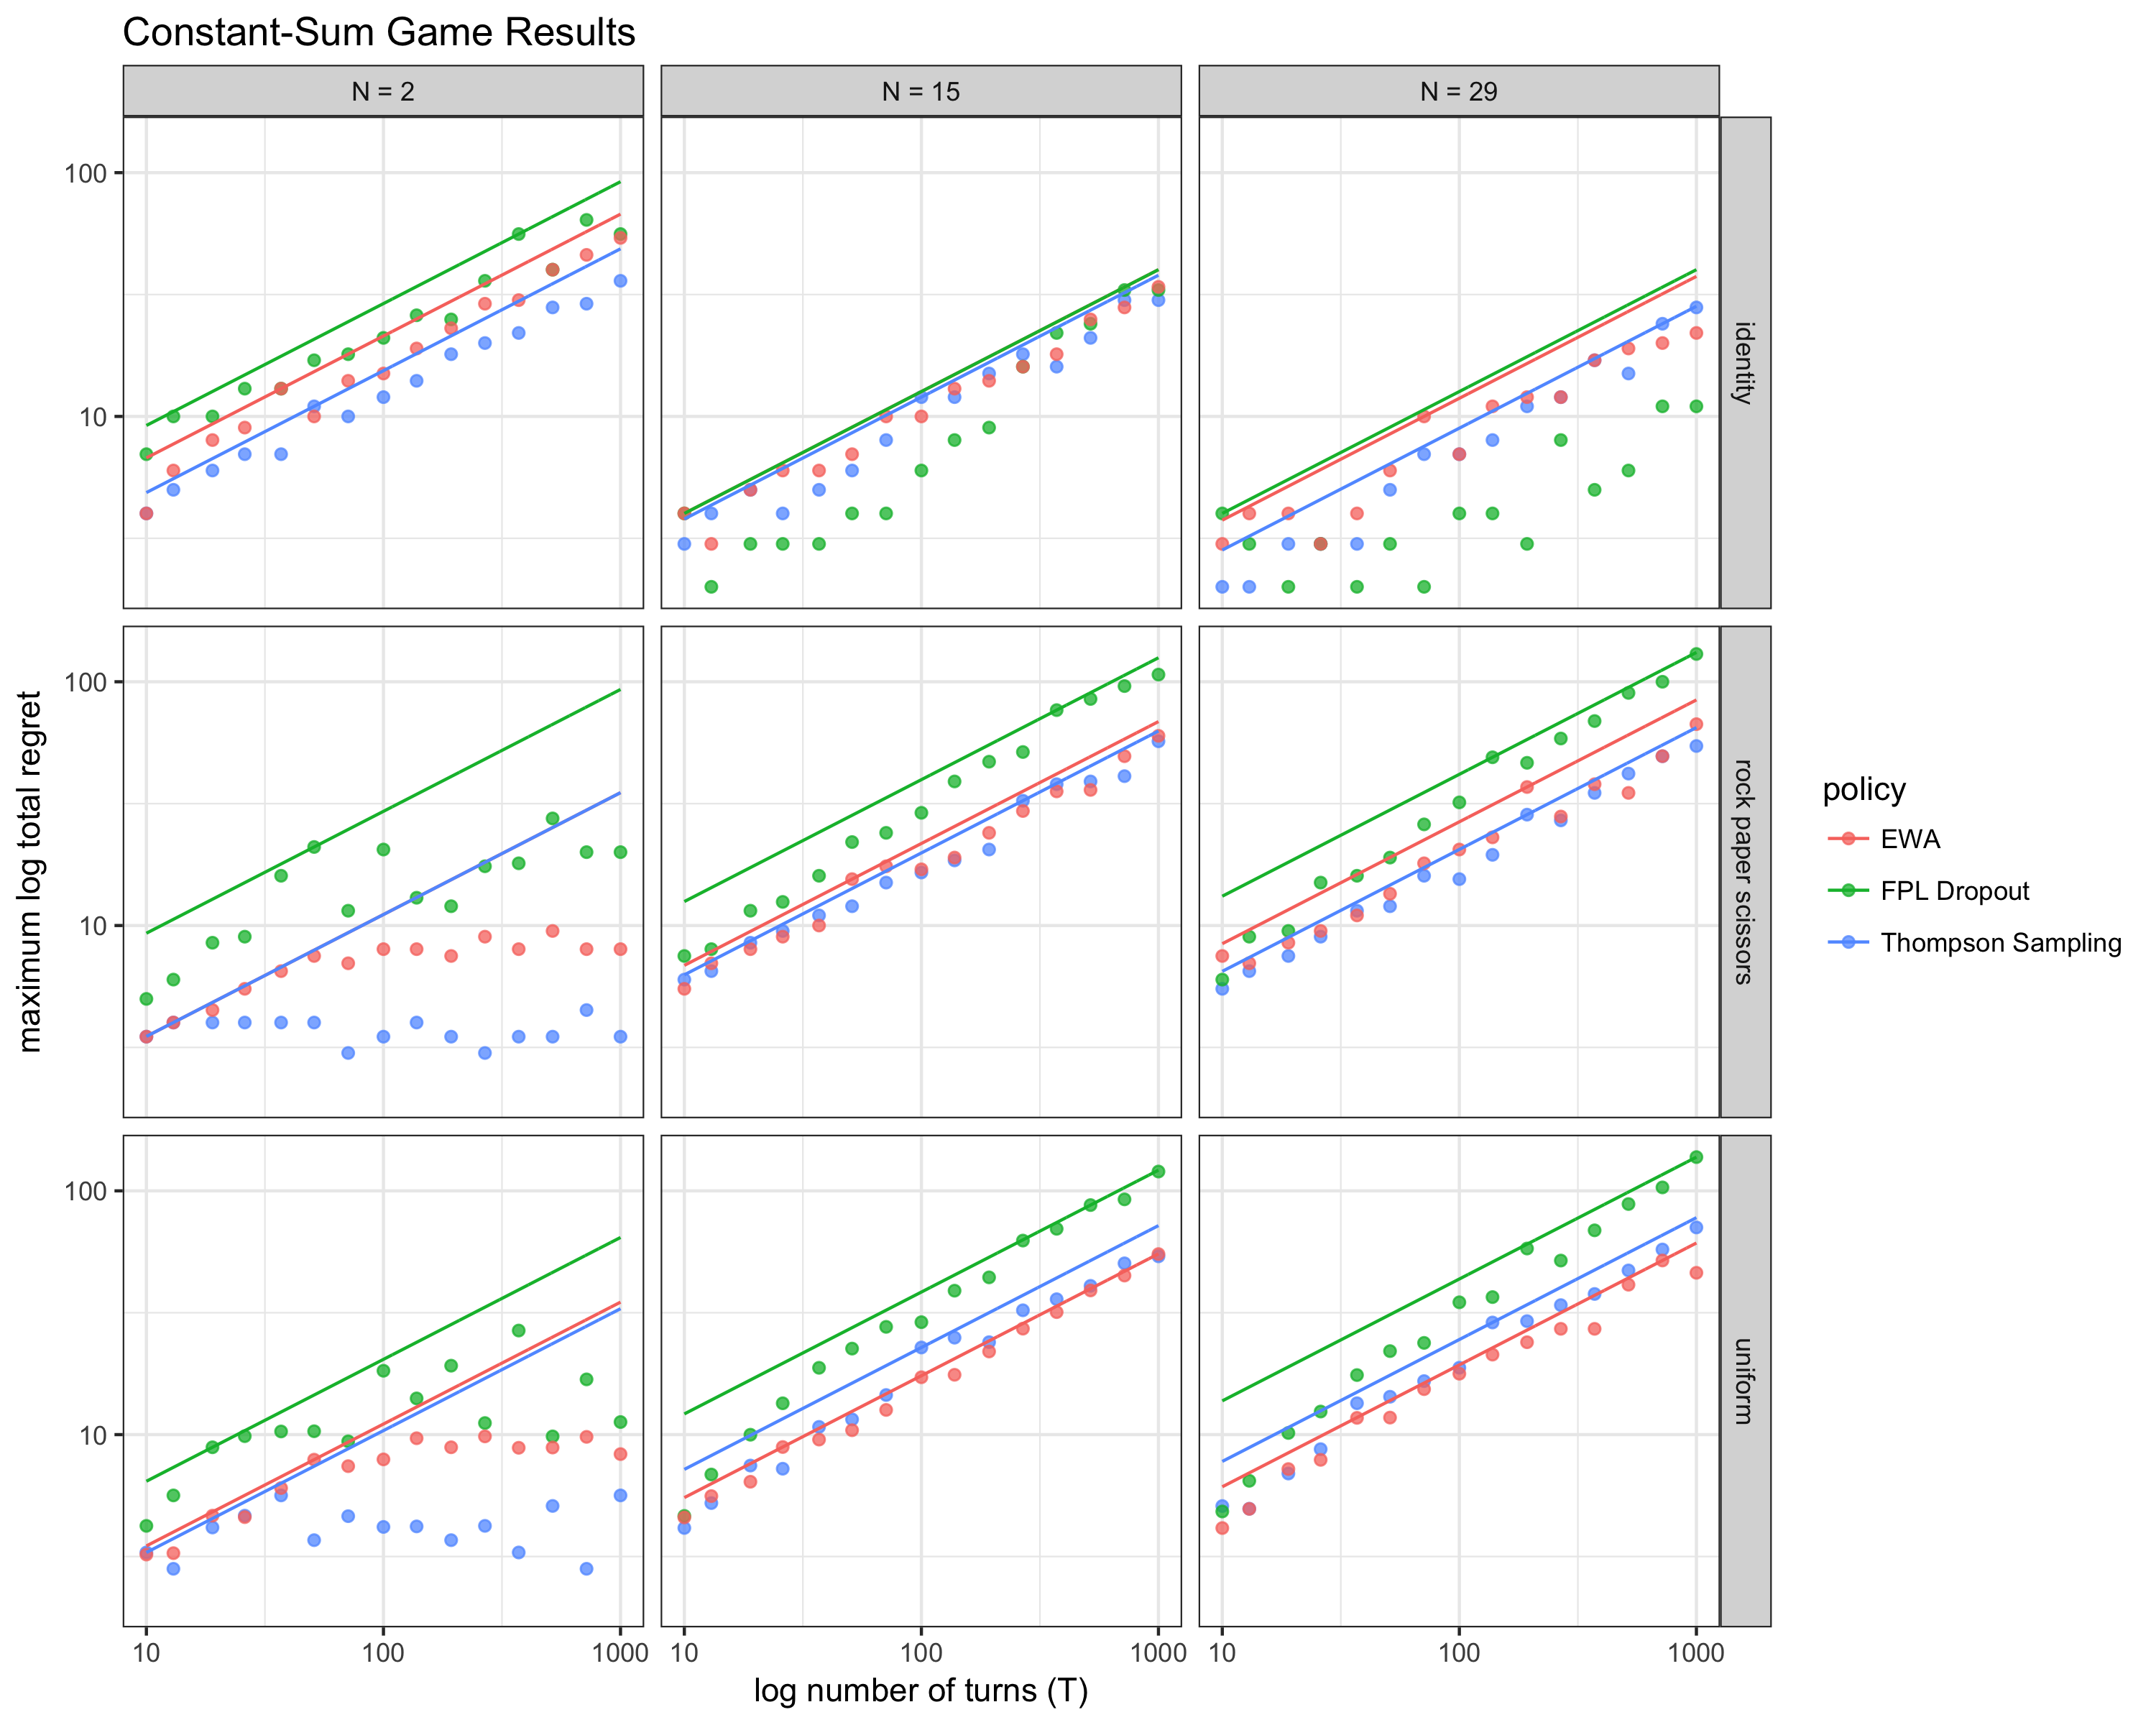
\includegraphics[width=1.5\textwidth]{../images/game_theory/num_turns_by_regret}
	}
	\end{figure}

	
	\pagebreak
	
	\section{Evolutionary Strategies}	
	
	In our quest for testing the limits of Thompson Sampling we now view our situation as an optimization problem which we explore with evolutionary strategies.  Recall the optimization problem we are trying to solve is $ \max_\ell E [R_T] $ where $\ell \in \left[ 0, 1 \right]^{N \times T} $.  Now, we play the role of adversary trying to maximize the forecaster's regret.  Since there is not a known closed form solution, we get creative and resort to evolutionary methods.
		
	These methods were inspired by Darwinian evolution and so the language is also quite biological.  An individual in this case is a possible loss matrix $\ell \in \left[ 0, 1 \right]^{N \times T} $.  We initialize a population of 100 by sampling this space uniformly at random.  We then estimate the regret by running the learning algorithm (i.e. Thompson Sampling) against this loss matrix twice.  Then we select only the top third to repopulate.  The others are discarded.  The individuals left have two children each generated by perturbing the loss matrix with Gaussian noise of variance $0.025$.  For one of the children, every entry is perturbed. For the other, only a quarter of the entries are perturbed.  For each generation, we test the fitness by estimating regret, sort the individuals by average regret, remove the two thirds of the population with low regret estimates, generate two children each for the remaining individuals.  We repeated this procedure about two thousand times.  A separate population, each of 100 individuals, is maintained for different values of $N, T$ and the different algorithms we test.
		
	Below we vizualize the results of these tests.  Each point represents an individual.  The maximum points of each population is bold.  The line represents $R = a \sqrt{T}$ where $a$ is a constant chosen such that the curve is greater than or equal to all trials 
	
		
	\begin{figure}[h!]
		\makebox[\textwidth][c]{
		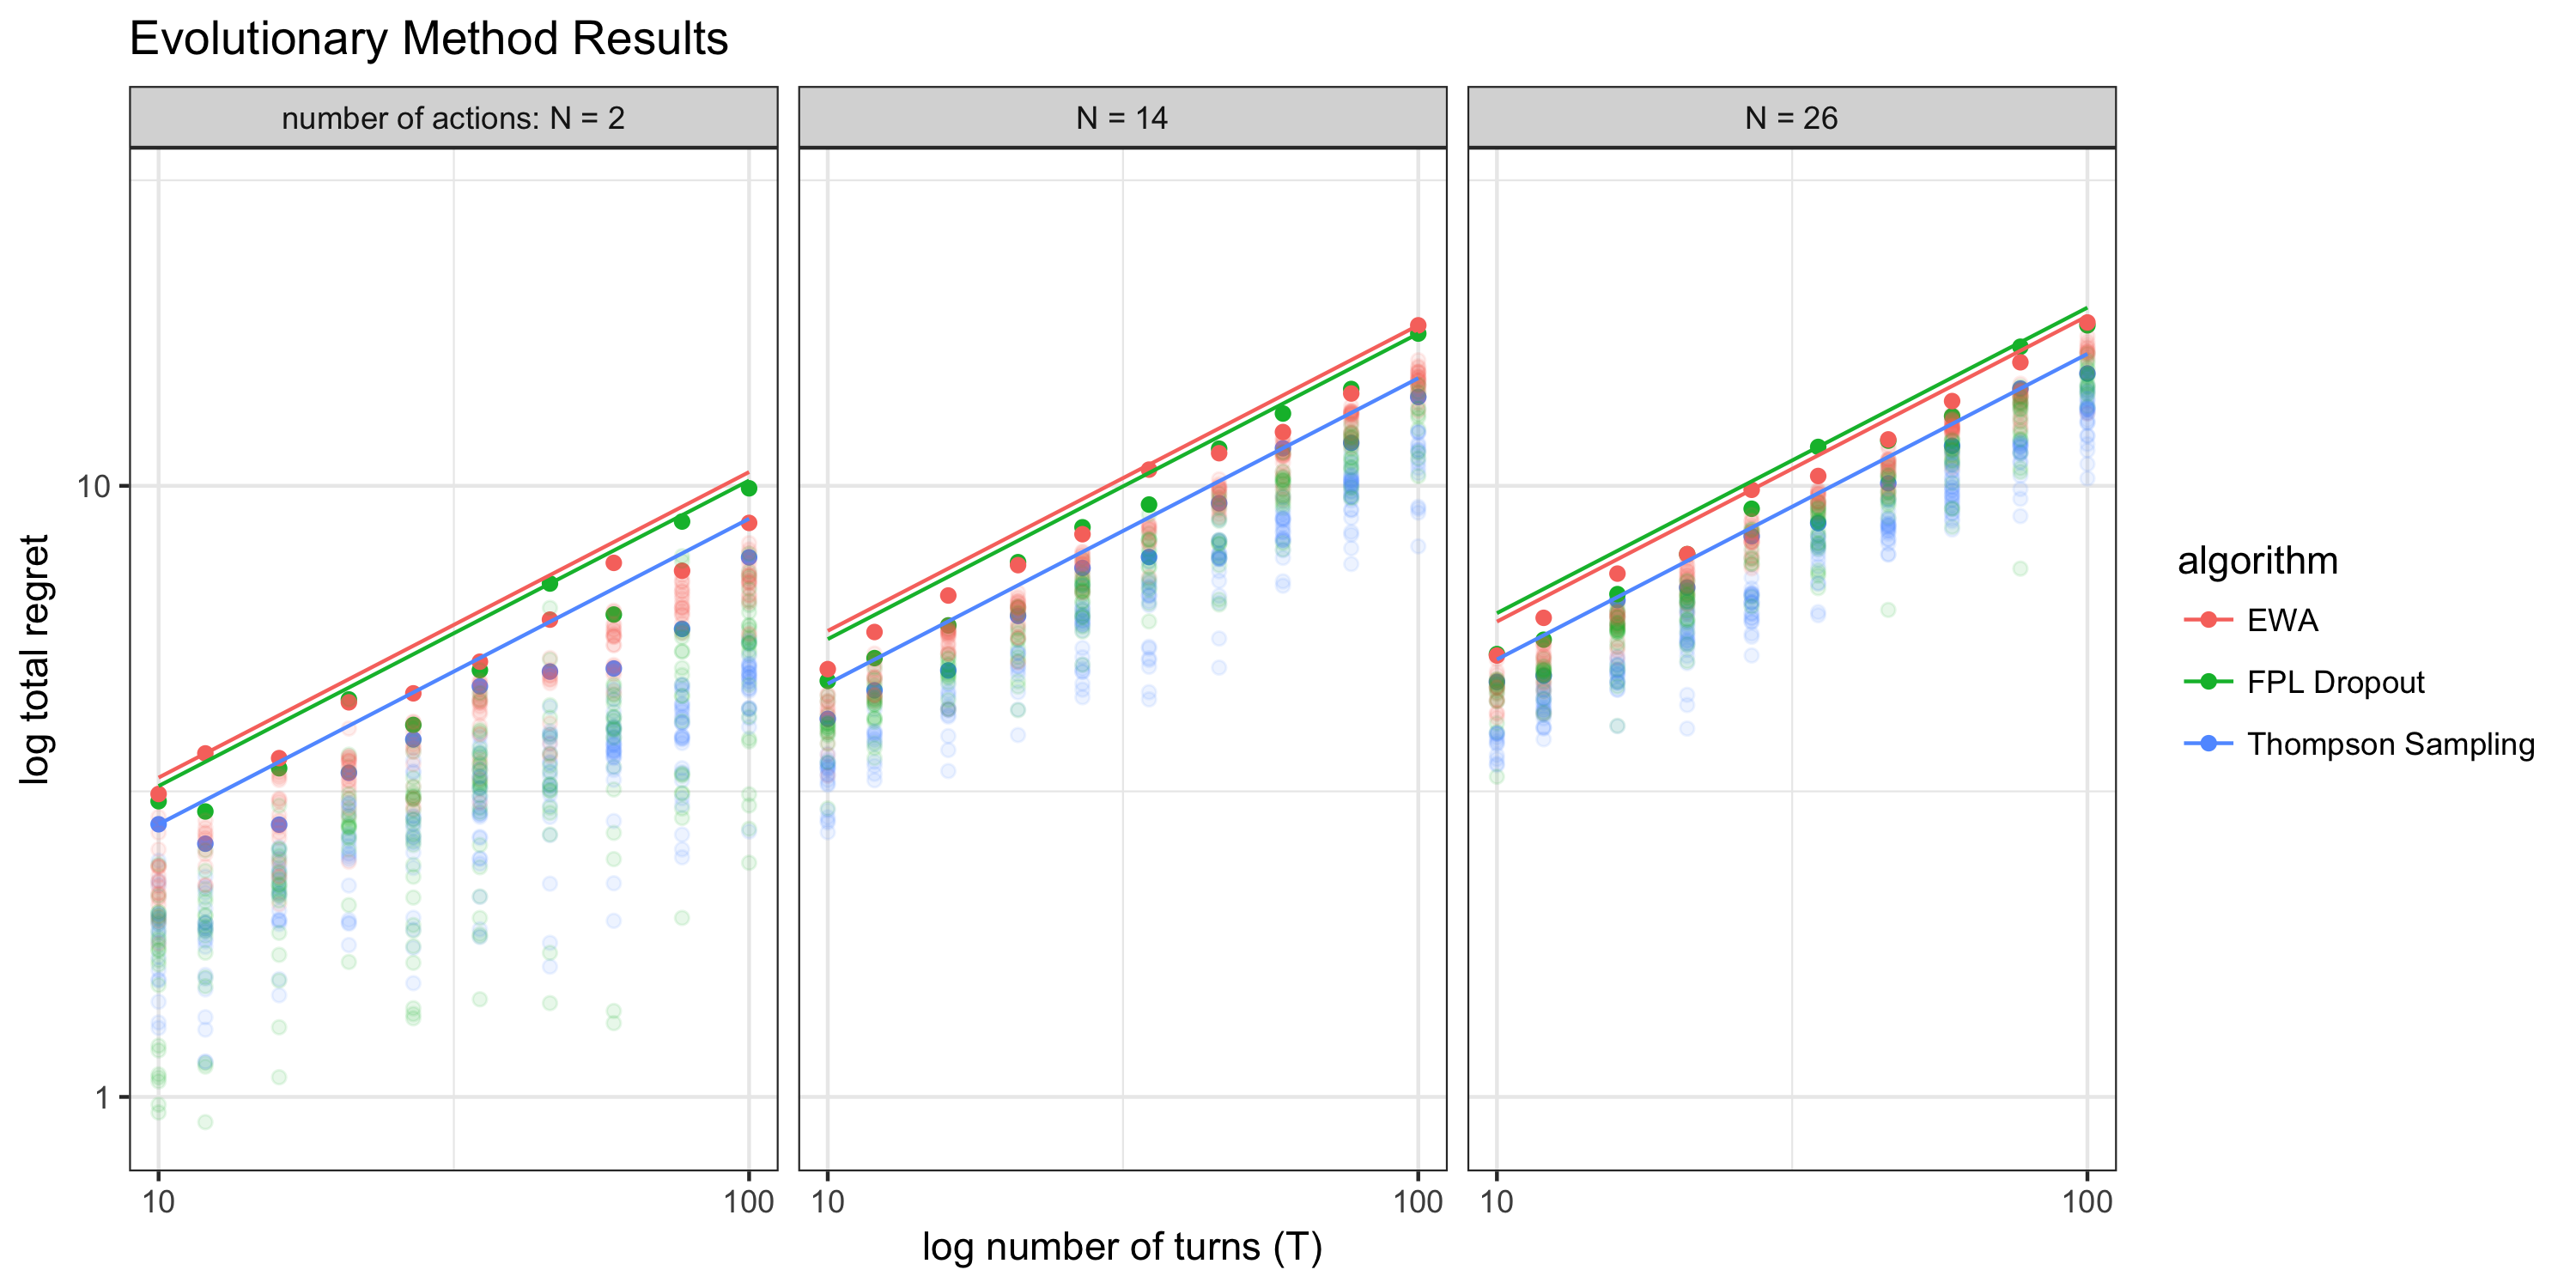
\includegraphics[width=1.4\textwidth]{../images/evolutionary/num_turns_by_regret}
	}
	\end{figure}

	In this setup Thompson Sampling consistently performs better than either of the other two algorithms.  While this does not prove any guaranteed regret bound on the algorithm (evolutionary algorithms have no guarantees to converge to a global optimum).  This is a strong indication that Thompson Sampling is a robust algorithm if it is able to outperform these other two provably robust algorithms.

	\section{Related Work}
	
	There are a few results in this domain worth mentioning.  The first of which is a paper by Gopalan from 2013 where he shows that Thompson Sampling with Gaussian prior and liklihood is exactly equivalent to Follow the Perturbed Leader with Gaussian perturbations \cite{FPL_TS_Gaussian}.  Thus, the regret bound on the FPL strategy can be transfered to Thompson Sampling.  In retrospect, is quite an intuitive result.  In Thompson Sampling the uncertainty is expressed as a posterior distribution. For FPL, it's a perturbation.  When they both have the same distribution, they are equivalent. 	An area of future exploration is if there are other similar connections to FPL when the priors have different distributions.
	
	Another mention of our problem is Russo et al.'s recent tutorial on Thompson Sampling \cite{Russo_TS}.  They discuss the case when losses are generated from a Bernoulli distribution whose parameter drifts with time.  They propose an alteration to the original Thompson Sampling where greater weight is given to data more recently seen.  This, however, is not the full adversarial framework we are after.

	\section{Conclusion}
	
	In this thesis we have provided empirical evidence that Thompson Sampling is robust in adversarial settings.  We compared it's performance with two provably robust algorithms: follow the perturbed leader and exponential weighted averaging in constant sum games and an evolutionary setting.  Thompson Sampling performed just as well, and sometimes better than these two algorithms.  Looking forward, hopefully this evidence will inspire a mathematical proof of an external regret bound.
	
	All of the code used in this thesis can be found at \url{github.com/TravisDunlop/thompson-sampling-thesis}
	
	
	% bib stuff
	\nocite{*}
	\bibliographystyle{plain}
	\bibliography{bibliography}
\end{document}